\documentclass[12pt,]{article}
\usepackage[left=1in,top=1in,right=1in,bottom=1in]{geometry}
\newcommand*{\authorfont}{\fontfamily{phv}\selectfont}
\usepackage{lmodern}


  \usepackage[T1]{fontenc}
  \usepackage[utf8]{inputenc}



\usepackage{abstract}
\renewcommand{\abstractname}{}    % clear the title
\renewcommand{\absnamepos}{empty} % originally center

\renewenvironment{abstract}
 {{%
    \setlength{\leftmargin}{0mm}
    \setlength{\rightmargin}{\leftmargin}%
  }%
  \relax}
 {\endlist}

\makeatletter
\def\@maketitle{%
  \newpage
%  \null
%  \vskip 2em%
%  \begin{center}%
  \let \footnote \thanks
    {\fontsize{18}{20}\selectfont\raggedright  \setlength{\parindent}{0pt} \@title \par}%
}
%\fi
\makeatother




\setcounter{secnumdepth}{0}


\usepackage{graphicx}
% We will generate all images so they have a width \maxwidth. This means
% that they will get their normal width if they fit onto the page, but
% are scaled down if they would overflow the margins.
\makeatletter
\def\maxwidth{\ifdim\Gin@nat@width>\linewidth\linewidth
\else\Gin@nat@width\fi}
\makeatother
\let\Oldincludegraphics\includegraphics
\renewcommand{\includegraphics}[1]{\Oldincludegraphics[width=\maxwidth]{#1}}

\title{Inaction on climate change could approach one year of life in some
European countries \thanks{All data and code that supports these conclusions are available as
supplementary materials.}  }



\author{\Large Mathew E. Hauer\textsuperscript{1}*\vspace{0.05in} \newline\normalsize\emph{University of Georgia}   \and \Large Alexis R. Santos\textsuperscript{2}\vspace{0.05in} \newline\normalsize\emph{Pennsylvania State University}  }


\date{}

\usepackage{titlesec}

\titleformat*{\section}{\normalsize\bfseries}
\titleformat*{\subsection}{\normalsize\itshape}
\titleformat*{\subsubsection}{\normalsize\itshape}
\titleformat*{\paragraph}{\normalsize\itshape}
\titleformat*{\subparagraph}{\normalsize\itshape}


\usepackage{natbib}
\bibliographystyle{apsr}
\usepackage[strings]{underscore} % protect underscores in most circumstances



\newtheorem{hypothesis}{Hypothesis}
\usepackage{setspace}

\makeatletter
\@ifpackageloaded{hyperref}{}{%
\ifxetex
  \PassOptionsToPackage{hyphens}{url}\usepackage[setpagesize=false, % page size defined by xetex
              unicode=false, % unicode breaks when used with xetex
              xetex]{hyperref}
\else
  \PassOptionsToPackage{hyphens}{url}\usepackage[unicode=true]{hyperref}
\fi
}

\@ifpackageloaded{color}{
    \PassOptionsToPackage{usenames,dvipsnames}{color}
}{%
    \usepackage[usenames,dvipsnames]{color}
}
\makeatother
\hypersetup{breaklinks=true,
            bookmarks=true,
            pdfauthor={Mathew E. Hauer\textsuperscript{1}* (University of Georgia) and Alexis R. Santos\textsuperscript{2} (Pennsylvania State University)},
             pdfkeywords = {Climate change, Life expectancy, Mortality, Demography, Excess
mortality, Europe, Public health},  
            pdftitle={Inaction on climate change could approach one year of life in some
European countries},
            colorlinks=true,
            citecolor=blue,
            urlcolor=blue,
            linkcolor=magenta,
            pdfborder={0 0 0}}
\urlstyle{same}  % don't use monospace font for urls

\usepackage[all]{nowidow}
\usepackage{rotating}
\usepackage{fancyhdr}
\usepackage[table]{xcolor}
\usepackage{tabularx}
\usepackage{makecell}
\usepackage{xcolor}
\pagestyle{fancy}
\fancyhead{}
\fancyhead[C]{Climate change life expectancy}


% add tightlist ----------
\providecommand{\tightlist}{%
\setlength{\itemsep}{0pt}\setlength{\parskip}{0pt}}

\begin{document}
	
% \pagenumbering{arabic}% resets `page` counter to 1 
%
% \maketitle

{% \usefont{T1}{pnc}{m}{n}
\setlength{\parindent}{0pt}
\thispagestyle{plain}
{\fontsize{18}{20}\selectfont\raggedright 
\maketitle  % title \par  

}

{
   \vskip 13.5pt\relax \normalsize\fontsize{11}{12} 
\textbf{\authorfont Mathew E. Hauer\textsuperscript{1}*} \hskip 15pt \emph{\small University of Georgia}   \par \textbf{\authorfont Alexis R. Santos\textsuperscript{2}} \hskip 15pt \emph{\small Pennsylvania State University}   

}

}








\begin{abstract}

    \hbox{\vrule height .2pt width 39.14pc}

    \vskip 8.5pt % \small 

\noindent Climate change related estimates of excess mortality clearly demonstrate
the dramatic impact on public health and human mortality from climate
change. However, life expectancy at birth is more easily communicated
and understood by the public, and controls for different geographic,
economic, and demographic groups. No studies have comprehensively
connected excess mortality due to climate change to anticipated
reductions in life expectancy. Without properly situating the potential
loss of life within the contexts of life expectancy, we risk
misrepresenting cost of climate change on mortality. In this paper, we
convert excess mortality estimates due to increaes in extreme weather
from climate change into potential reductions of life expectancy at
birth and report the cost of climate change on human longevity. We find
climate change extremes could become the third largest life expectancy
reducer behind heart disease and cancer in some European countries.
Thus, the cost of inaction on climate change could approach one year of
life in some countries and possibly exceed that.


\vskip 8.5pt \noindent \emph{Keywords}: Climate change, Life expectancy, Mortality, Demography, Excess
mortality, Europe, Public health \par

    \hbox{\vrule height .2pt width 39.14pc}



\end{abstract}


\vskip 6.5pt


\noindent \doublespacing \begin{itemize}
\tightlist
\item
  Corresponding author.
  \href{mailto:hauer@uga.edu}{\nolinkurl{hauer@uga.edu}}. p:
  706-542-9369.
\end{itemize}

\textsuperscript{1} Department of Sociology, Florida State University.
201 N. Milledge Ave. Athens, GA USA 30602.

\textsuperscript{2} Department of Sociology and Criminology,
Pennsylvania State University. 901 Oswald Tower, University Park, PA USA
16802.

\newpage

\hypertarget{main-text}{%
\section{Main Text}\label{main-text}}

Climate change's implications on humanity go far beyond estimates of
economic damages \citep{hsiang2017estimating}, estimates of displacement
\citep{rigaud2018groundswell}, or human conflict
\citep{barnett2007climate} but have the potential to lead to the loss of
human life \citep{forzieri2017increasing, pachauri2014climate}. As
impact quantification studies move further from the physical sciences of
climate change into the social sciences, properly quantifying and
conveying the impact of climate change on public health is of increasing
importance \citep{melillo2014climate, cloyd2016engagement}.

Scholars have long estimated the mortality risks associated with climate
change and typically use excess or extra mortality
\citep{forzieri2017increasing, wilson2017climate, mcmichael2006climate, zanobetti2012summer}.
Although such estimates are useful, the excess mortality estimates are
rather sterile -- one death is a tragedy, a million deaths a statistic
-- and difficult to relate to on an individual level. Life expectancy at
birth (\(e_0\)), on the other hand, provides potent comparisons of
mortality vectors and converts excess mortality into an intuitively
understood metric, relatable to everyone. To our knowledge, no studies
exist that comprehensively examine the potential reductions of life
expectancy due to climate change. Without properly situating the
potential loss of life within the contexts of metrics such as life
expectancy, we risk underestimating the impact of climate change on
human mortality.

Using published data on excess mortality \citep{forzieri2017increasing},
we connect climate change excess mortality to life expectancy in a
mortality model. By estimating the increase in age-specific mortality
rates associated with previously published excess death estimates, we
can assess how much climate change could reduce the anticipated
longevity of the average person in twenty-eight European countries. This
approach allows us to quantify the impact of climate change on human
longevity and answer the following questions: What is the cost of
inaction on climate change on human longevity? and How does climate
change related mortality compare to other mortality vectors? Our results
situate climate change mortality within the broader context of human
mortality and can be used to inform public health interventions to
prevent such futures.

Our results suggest that climate change could emerge as a potent new
mortality vector in the 20th century. Mitigation strategies (ie
reductions in greenhouse gas emisions) and adaptation strategies (ie
outreach efforts, retrofitting public buildings, etc.) would help
prevent this new public health concern.

\hypertarget{background}{%
\section{Background}\label{background}}

\hypertarget{climate-change-and-human-mortality}{%
\subsection{Climate change and human
mortality}\label{climate-change-and-human-mortality}}

\hypertarget{methods-and-materials}{%
\section{Methods and Materials}\label{methods-and-materials}}

We estimate changes in life expectancy by combining three primary
datasets: excess mortality data due to meterological hazards related to
climate change from Forzieri et al. \citep{forzieri2017increasing},
cause-of-death distributions from the Global Burden of Disease study
(GBD) \citep{GBD, wang2012age}, and life tables from the Human Mortality
Database (HMD) \citep{HMD}. Forzieri et al.
\citep{forzieri2017increasing} focused on the projected excess mortality
of heatwaves, coldwaves, wildfires, droughts, river and coastal floods,
and windstorms under the business-as-usual greenhouse gas emission
scenario (SRES A1B). They modelled long-term, small-area demographic
changes in European countries that correspond to a middle-of-the-road
socioeconomic scenario (SSP2 with medium fertility, medium mortality,
medium migration, and the Global Education Trend education scenario) and
based their projected mortality on extrapolations of an exhaustive
examination of contemporary disaster databases within spatially
rectified, high-resolution gridded datasets. While the disaster data are
not standardized across country, Forzeri et al.~imputed data in
incomplete time periods and countries. This imputation could mask
spatial variability at the sub-national level, but here we use their
country-aggregated results. Their results represent business-as-usual
climate change and human development without incorporating potential
adaptation. They found a potential 150,000+ climate change related
fatalities per year by the mid 2080s with climate change contributing to
90\% of mortality rise as opposed to population changes. These data
provide the anticipated fatalities but not the effect these deaths might
have on life expectancy.

To convert excess mortality to life expectancy, we use data gathered
from the HMD \citep{HMD} for corresponding European countries in
five-year life tables in conjunction with cause-specific mortality data
from the GBD \citep{GBD, wang2012age}. The HMD comprises only complete,
official vital event statistics and represents the most accurate and
complete compilation of mortality data available. We allocate excess
multi-hazard mortality for each country from supplementary table S8 in
Forzieri et al. \citep{forzieri2017increasing} based on the observed
mortality schedule for environmental heat and cold exposure deaths from
the GBD for each country in the previous decade.

\begin{table}
\caption{\textbf{Most recent mortality data available by country in the HMD.}} \label{Table2}
\begin{tabular}{ll|ll|ll|ll}
Country & Year & Country & Year & Country & Year & Country & Year \\
\hline
AUT     & 2014 & ESP     & 2014 & HUN     & 2014 & NLD     & 2016 \\
BEL     & 2015 & EST     & 2014 & IRL     & 2014 & NOR     & 2014 \\
BGR     & 2010 & FIN     & 2015 & ISL     & 2016 & POL     & 2014 \\
CHE     & 2016 & FRATNP  & 2015 & ITA     & 2014 & PRT     & 2015 \\
CZE     & 2016 & GBR     & 2016 & LTU     & 2014 & SVK     & 2014 \\
DEUT    & 2015 & GRC     & 2013 & LUX     & 2014 & SVN     & 2014 \\
DNK     & 2016 & HRV     & 2016 & LVA     & 2014 & SWE     & 2016 \\
\hline
\end{tabular}
\end{table}

We then recalculated age-specific mortality rates in five-year life
tables by adding the climate change mortality onto the underlying
mortality data and create four subsequent life tables (\(baseline\),
\(low\), \(mid\), \(high\)) using standard life table techniques
\citep{wunsch2013life} based on the published confidence intervals from
\citep{forzieri2017increasing}. We used a variant of the cause-deleted
life tables approach
\citep{brand2005approximations, beltran2008integrated} to measure the
impact of excess mortality on life expectancy at birth or \(e_0\).
Changes in life expectancy are reported based on differentials from
\(e_0\) between the 2080s and the most recent complete life table in the
HMD (see \textbf{Table 1} for the years used). Complete life tables for
all countries are available in the \emph{Supplementary Dataset} and all
computer code to replicate our results are available online\footnote{Replication
  files are located here:
  \url{https://osf.io/fp52x/?view_only=754d9a72a2ea4f6b8e0c193dc9a590d1}}.

\hypertarget{data}{%
\subsection{Data}\label{data}}

To create life expectancy differentials, we used three sources of data.
The first is the baseline life table data. Baseline life tables comes
from the Human Mortality Database (HMD) \citep{HMD}. These datasets
comprise only official vital event registration and are considered the
most complete and accurate source of mortality data available. We
downloaded the most recent 5x1 (by age and year) life table data for
twenty-eight European countries. We used the following data elements
from the five-year age group life table data in the HMD:

\begin{enumerate}
\item $_nP_x$ or the population in age group $x$ for $n$-year intervals from exact age $x$ to $x+n$.
\item $_na_x$ or the average length of survival between ages $x$ and $x+n$.
\item $_nd_x$ or the number of deaths in age group $x$ for $n$-year intervals from exact age $x$ to $x+n$.
\end{enumerate}

The second dataset comes from published projections of climate-related
mortality in Europe \citep{forzieri2017increasing}. Forzieri et al.
\citep{forzieri2017increasing} combined data from the International
Disaster Database (EMCAT) and the Natural Catastrophe Statistics tool
(NatCatSERVICE) to create exposure and fatality statistics related to
six weather-related hazards -- heatwaves, cold waves, droughts,
wildfires, river and coastal floods, and windstorms. They downscaled
these exposures to 1km grid scales and integrated them into small-area
demographic projections for Europe out to 2100. Heatwaves and coldwaves
account for the vast majority of projected fatalities. The number of
future anticipated deaths are available in their Supplementary Table S8
\citep{forzieri2017increasing} and provide the magnitude of deaths for
our study.

The third dataset comes from the GBD \citep{GBD, wang2012age}. The GBD
is the most comprehensive worldwide dataset of epidemiological data
produced and provides cause-specific mortality by age/sex/geography/year
for 249 causes of death in 195 countries and territories. We gathered
data on age-specific deaths and mortality rates (\(m_x\)) for mortality
from environmental heat and cold exposure (cause C.2.9) for the period
2006-2015 for each country in the study. These data provide a mortality
schedule to fit the projected climate change excess mortality from
Fozieri et al \citep{forzieri2017increasing}. Thus, we assume that the
age-specific mortality schedules observed between 2006 and 2015 due to
environmental heat and cold exposure in the GBD (see \autoref{suppfig})
are likely to remain unchanged in the future.

\begin{figure}
\centering
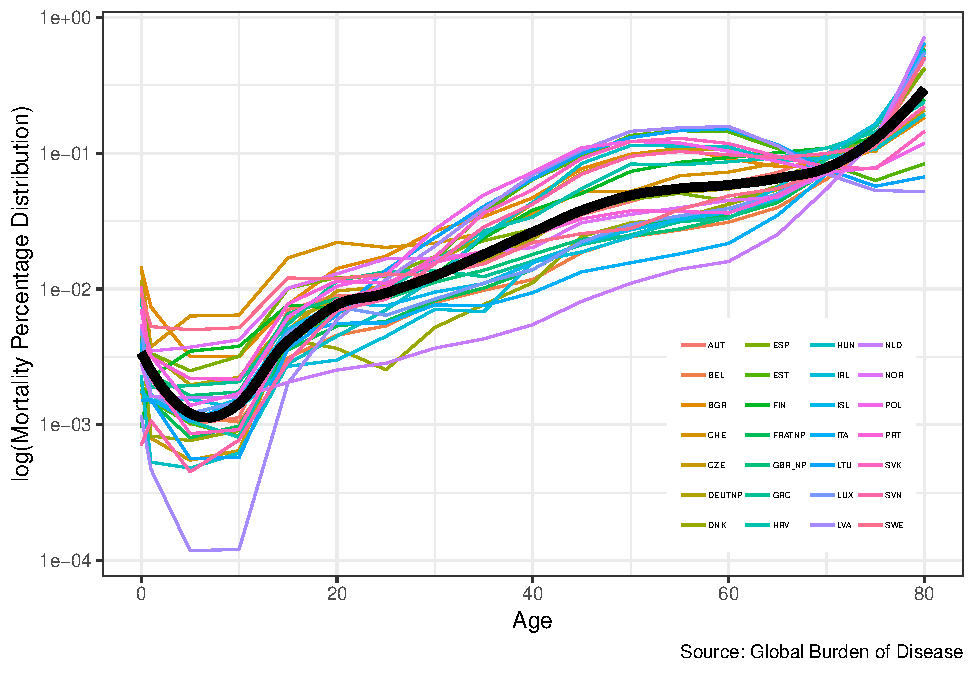
\includegraphics{MS-cclifeexpec_files/figure-latex/suppfig-1.pdf}
\caption{\textbf{Mortality distribution of Heat-related mortality in 28
European countries}. The thick black line is the average\label{suppfig}}
\end{figure}

\hypertarget{methods}{%
\subsection{Methods}\label{methods}}

We derived a number of additional variables to accomplish our analysis.
First, we abridged the life table data from the HMD from ages 100+ to
80+ to conform to the GBD cause-specific mortality schedules.

From the GBD data, we derived variable \(t_{x,i}\) as the proportion of
deaths, \(D\), from each age group \(x\) in each country \(i\)
(\(_nt_{x,i}=D_{x,i}^{GBD}/\sum_{\alpha=0}^{80}{_nD_{\alpha,i}^{GBD}}\)).

We then derived additional \(m_x\) rates for each age group \(x\) in
each country \(i\) for each scenario \(s\) (\(BASE\), \(LOW\), \(MID\),
\(HIGH\)) from Forzieri et al \citep{forzieri2017increasing}.

\begin{equation}
_nm_{x,i,BASE} = _nD_{x,i}^{HMD} \,/\, _nP_{x,i}^{HMD}
\end{equation}

\begin{equation}
_n\hat{m}_{x,i,s} = (_nD_{x,i}^{HMD} + (\hat{D_{i,s}} \,\cdot\, _nt_{x,i}) ) \,/\, _nP_{x,i}^{HMD}
\end{equation}

where \(D_{x,i}\) is the number of deaths in age group \(x\) in country
\(i\) from the HMD, \(P_{x,i}\) is the population in age group \(x\)
from the HMD, \(\hat{D_{i,s}}\) is the number of deaths from Forzieri et
al. \citep{forzieri2017increasing} under scenario s, and \(t_{x,i}\) is
the proportion of mortality experienced in each age group \(x\) from the
GBD. Thus, the anticipated additional mortality due to climate change is
added to each age group based on the underlying cause-specific mortality
schedule observed between 2006-2015 in the GBD.

We then calculated \(q_x\) values, or the probability of dying, for each
scenario \(s\) for each country.

\begin{equation}
_nq_{x,i,BASE} = \frac{m_{x,i,BASE}}{1+(n-_na_{x,i}) \cdot m_{x,i,BASE}}
\end{equation}

\begin{equation}
_n\hat{q}_{x,i,s} = \frac{\hat{m}_{x,i,s}}{1+(n-_na_{x,i}) \cdot \hat{m}_{x,i,s}}
\end{equation}

We calculated each additional life table value identically for each
scenario \(s\) using standard life table equations:

\[_nd_{x,i,s} = _nl_{x,i,s} \cdot _nq_{x,i,s}\]
\[_nl_{x,i,s} = _nl_{x-1,i,s} - _nd_{x-1,i,s}\]
\[_nL_{x,i,s} = _na_{x,i,s} \cdot _nl_{x,i,s} + ((n-_na_{x,i,s}) \cdot _nl_{x,i,s})\]
\[_nT_{x,i,s} = _nL_{x,i,s} + _nT_{x+1,i,s}\]
\[_ne_{x,i,s} = _nT_{x,i,s} / _nl_{x,i,s}\]

To determine the differences between life expectancy compared to the
baseline, we simply subtract \(e_{x,i,s}\) (for scenario \(LOW\),
\(MID\), and \(HIGH\)) from \(e_{x,i,BASE}\) as described by
\citep{beltran2008integrated}.

\hypertarget{results}{%
\section{Results}\label{results}}

We find that climate change could alter life expectancy by -0.23 years
(-2.5 months (-0.1 to -0.39 years)) in the average European country
(\textbf{\autoref{figure1}}). This reduction is comparable to mortality
due to influenza and pneumonia \citep{arias2013united} in the United
States for the year 2000. Although the average European country could
see a change of -0.23 years, several countries are likely to experience
considerably greater reductions in life expectancy. Luxembourg could see
a reduction of up to 2.2 years and the medium-variant of climate hazards
could cost the average Spaniard 1.03 years of life.

\begin{figure}
\centering
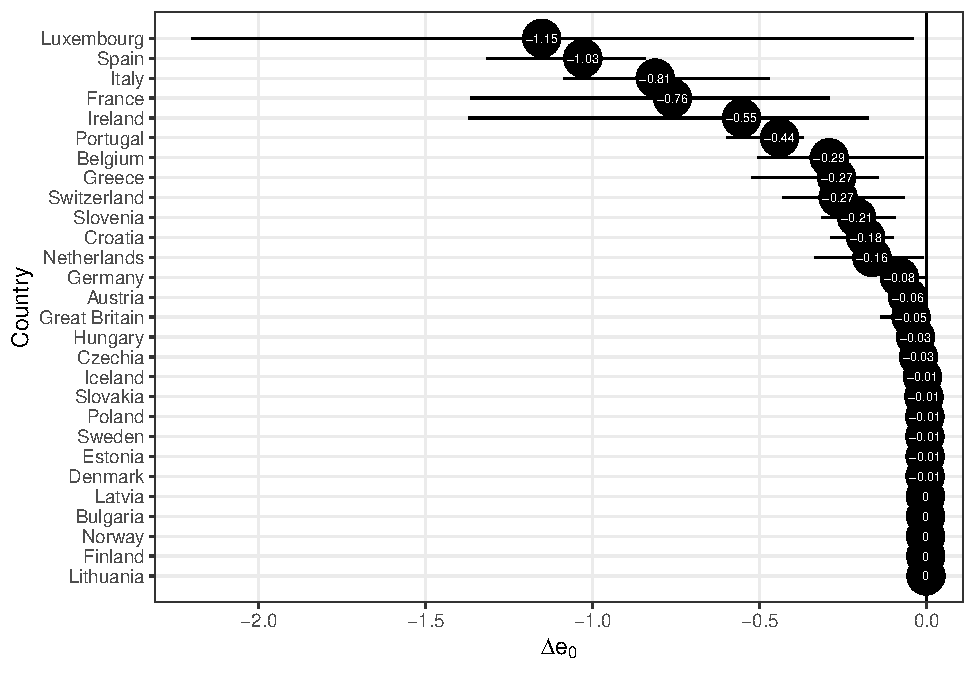
\includegraphics{MS-cclifeexpec_files/figure-latex/figure1-1.pdf}
\caption{Change in life expectancy at birth (\(e_0\)) due to
business-as-usual climate change in the 2080s compared to the present
\(e_0\). We report changes in life expectancies due to climate change
for twenty-eight European countries. The central values represent the
ensemble median while the stems represent the upper and lower bounds of
the inter-model climate variability.\label{figure1}}
\end{figure}

Our results also suggest climate change mortality differentials are
likely to unfold along highly uneven geographies (\autoref{map}).
Whereas many Northern European countries could experience negligible
impacts on life expectancy, five European countries could see life
expectancy changes in excess of -0.5 years (Spain, Luxembourg, France,
Italy, and Ireland). This group of countries could see life expectancy
changes of more than -1.0 years if climate change hazards are more
intense than anticipated. In some countries, climate change could thus
become a bigger killer than trachea, bronchus, and lung malignant
neoplasms (-0.85 years), acute myocardial infarction (-0.87 years), or
all accident related mortality (-0.84 years) \citep{arias2013united} by
the end of the century.

\begin{figure}
\centering
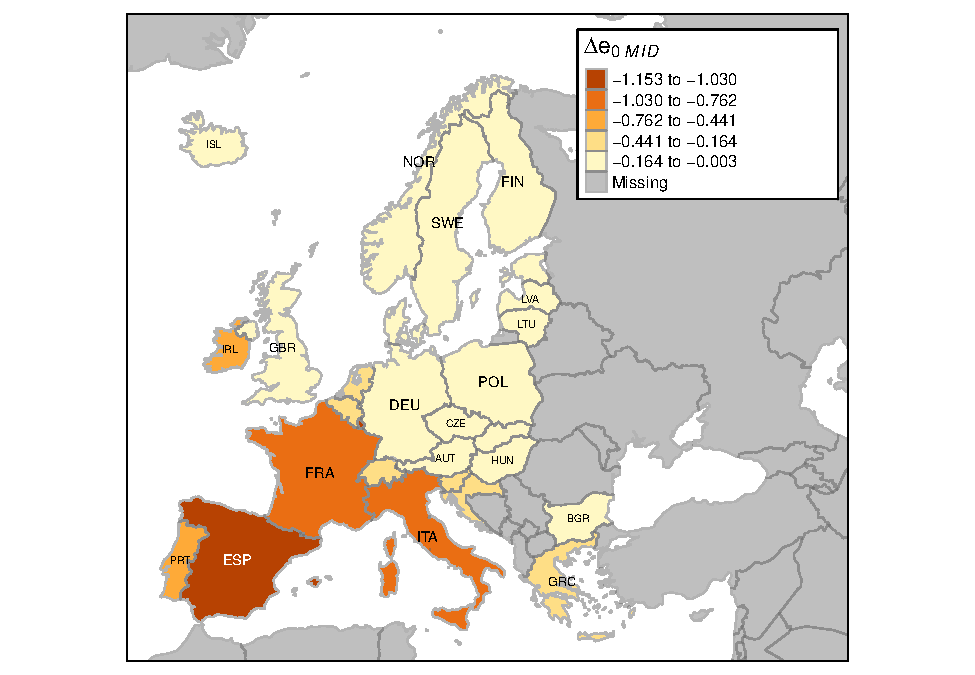
\includegraphics{MS-cclifeexpec_files/figure-latex/figure2-1.pdf}
\caption{Estimated reduction in life expectancy at birth (\(e_0\)) by
the 2080s under the \(MID\) scenario.\label{map}}
\end{figure}

\textbf{\autoref{Table1}} reports the rankings of Age Standardised Death
Rates (ASDR) for the leading causes of death in these European countries
(ASDR's for other CODs come from Eurostat (online data code:
hlth\_cd\_asdr2)) with our estimates of climate change included. In many
European countries, climate change could emerge as a top five killer.
Only combined CODs, such as all circulatory diseases or all cancers,
exhibit higher ASDRs if climatic hazards are more severe than
anticipated for Spain, Luxembourg, and France.

While Forzieri et al's \citep{forzieri2017increasing} results suggest
that the greatest climate change related mortality will unfold along a
north-south gradient, we find the greatest reduction in life expectancy
unfolds along an east-west gradient (\textbf{\autoref{map}}). The most
westerly European countries tend to have the greatest reductions.
Neighboring pairs of countries at similar latitudes could experience
vastly different mortality regimes, but neighboring pairs of countries
at similar longitudes seem to experience more similar mortality regimes
from climate change. Emergent research in Atmospheric Rivers suggest
Western Europe could be more susceptible to these types of events
\citep{ramos2015daily}. Additionally, these results point to the
importance of converting excess mortality into life expectancy to
properly quantify the effects of climate change mortality.

\hypertarget{discussion}{%
\section{Discussion}\label{discussion}}

In this article, we demonstrate the impact climate change could have on
life expectancy at birth in twenty-eight European countries. Previous
studies on climate change and excess mortality potentially
miscommunicate the impact climate change could have on human mortality.
Contrary to excess mortality estimates, life expectancy is routinely
used as a primary metric for communicating overall health outcomes and
enjoys widespread use by major international organizations
\citep{world2015world, marmot2012building, salomon2012healthy}. Life
expectancy and its derivatives are the recommended metrics for
population health \citep{parrish2010peer}. Additionally, it connects
mortality estimates into intuitively understandable metrics, translating
global estimates of mortality into individual outcomes. Our work reveals
the extent to which climate change could reduce the average person's
longevity by the end of the century, expanding our understanding of
climate change and public health; thus linking two of the major areas in
current developmental and sustainability discussion at both national and
international levels \citep{abel2016meeting}.

\begin{sidewaystable}

\caption{\textbf{Rankings of major causes of death in select European Countries based on a standardised death rate (per 100,000 inhabitants).} Data for other causes of death comes from Eurostat.} \label{Table1}
\rowcolors{2}{gray!25}{white}
\small
\begin{tabularx}{\textwidth}{l|XXXXXXXXX}
  \hline
   \rowcolor{white}
 Country & 1 & 2 & 3 & 4 & 5 & 6 & 7 & 8 \\ 
  \hline
Spain & \makecell{Respiratory\\Diseases\\ 91.7} & \cellcolor{blue!25}\makecell{\cellcolor{blue!25}Climate\\\cellcolor{blue!25}Change\\\cellcolor{blue!25} 78.05\\\cellcolor{blue!25}\begin{tiny}(63.26 - 101.6)\end{tiny}} & \makecell{Heart\\Disease\\ 68.2} & \makecell{Dis. of the\\Nervous Sys\\ 48.5} & \makecell{Lung\\Cancer\\ 47.8} & \makecell{Colorectal\\Cancer\\ 33.6} & \makecell{Suicide\\ 8.2} & \makecell{Transport\\Accidents\\ 4.3} \\ 
Luxembourg & \makecell{Heart\\Disease\\ 80.3} & \cellcolor{blue!25}\makecell{\cellcolor{blue!25}Climate\\\cellcolor{blue!25}Change\\\cellcolor{blue!25} 76.93\\\cellcolor{blue!25}\begin{tiny}(2.36 - 160.9)\end{tiny}} & \makecell{Respiratory\\Diseases\\ 63.8} & \makecell{Lung\\Cancer\\ 59.6} & \makecell{Dis. of the\\Nervous Sys\\ 38} & \makecell{Colorectal\\Cancer\\ 25.5} & \makecell{Suicide\\ 13.4} & \makecell{Transport\\Accidents\\ 6} \\ 
Italy & \makecell{Heart\\Disease\\ 98.3} & \makecell{Respiratory\\Diseases\\ 58.3} & \cellcolor{blue!25}\makecell{\cellcolor{blue!25}Climate\\\cellcolor{blue!25}Change\\\cellcolor{blue!25} 49.87\\\cellcolor{blue!25}\begin{tiny}(28.15 - 68.2)\end{tiny}} & \makecell{Lung\\Cancer\\ 49.4} & \makecell{Dis. of the\\Nervous Sys\\ 34.3} & \makecell{Colorectal\\Cancer\\ 27} & \makecell{Suicide\\ 6.3} & \makecell{Transport\\Accidents\\ 5.6} \\ 
France & \makecell{Respiratory\\Diseases\\ 52} & \makecell{Dis. of the\\Nervous Sys\\ 50.2} & \makecell{Lung\\Cancer\\ 50.1} & \cellcolor{blue!25}\makecell{\cellcolor{blue!25}Climate\\\cellcolor{blue!25}Change\\\cellcolor{blue!25} 49.61\\\cellcolor{blue!25}\begin{tiny}(18.24 - 93.5)\end{tiny}} & \makecell{Heart\\Disease\\ 49.3} & \makecell{Colorectal\\Cancer\\ 26.1} & \makecell{Suicide\\ 14.1} & \makecell{Transport\\Accidents\\ 5.1} \\ 
Portugal & \makecell{Respiratory\\Diseases\\ 116.7} & \makecell{Heart\\Disease\\ 69.6} & \makecell{Lung\\Cancer\\ 36.4} & \cellcolor{blue!25}\makecell{\cellcolor{blue!25}Climate\\\cellcolor{blue!25}Change\\\cellcolor{blue!25} 35.95\\\cellcolor{blue!25}\begin{tiny}(29.93 - 49.4)\end{tiny}} & \makecell{Colorectal\\Cancer\\ 35} & \makecell{Dis. of the\\Nervous Sys\\ 32.8} & \makecell{Suicide\\ 11.3} & \makecell{Transport\\Accidents\\ 7.8} \\ 
Ireland & \makecell{Heart\\Disease\\ 147.5} & \makecell{Respiratory\\Diseases\\ 125.9} & \makecell{Lung\\Cancer\\ 61.5} & \makecell{Dis. of the\\Nervous Sys\\ 48.7} & \cellcolor{blue!25}\makecell{\cellcolor{blue!25}Climate\\\cellcolor{blue!25}Change\\\cellcolor{blue!25} 44.65\\\cellcolor{blue!25}\begin{tiny}(13.57 - 119.6)\end{tiny}} & \makecell{Colorectal\\Cancer\\ 32.4} & \makecell{Suicide\\ 11} & \makecell{Transport\\Accidents\\ 4} \\ 
Slovenia & \makecell{Heart\\Disease\\ 102.8} & \makecell{Respiratory\\Diseases\\ 66.3} & \makecell{Lung\\Cancer\\ 58.6} & \makecell{Colorectal\\Cancer\\ 38.4} & \cellcolor{blue!25}\makecell{\cellcolor{blue!25}Climate\\\cellcolor{blue!25}Change\\\cellcolor{blue!25} 25.02\\\cellcolor{blue!25}\begin{tiny}(11.19 - 37.8)\end{tiny}} & \makecell{Dis. of the\\Nervous Sys\\ 21.1} & \makecell{Suicide\\ 18.9} & \makecell{Transport\\Accidents\\ 6.7} \\ 
Croatia & \makecell{Heart\\Disease\\ 306.5} & \makecell{Lung\\Cancer\\ 65.2} & \makecell{Respiratory\\Diseases\\ 59.7} & \makecell{Colorectal\\Cancer\\ 51} & \cellcolor{blue!25}\makecell{\cellcolor{blue!25}Climate\\\cellcolor{blue!25}Change\\\cellcolor{blue!25} 24.44\\\cellcolor{blue!25}\begin{tiny}(13.32 - 38.6)\end{tiny}} & \makecell{Dis. of the\\Nervous Sys\\ 21.3} & \makecell{Suicide\\ 16.8} & \makecell{Transport\\Accidents\\ 8.9} \\ 
Switzerland & \makecell{Heart\\Disease\\ 97.8} & \makecell{Respiratory\\Diseases\\ 51.3} & \makecell{Dis. of the\\Nervous Sys\\ 44.5} & \makecell{Lung\\Cancer\\ 42.1} & \cellcolor{blue!25}\makecell{\cellcolor{blue!25}Climate\\\cellcolor{blue!25}Change\\\cellcolor{blue!25} 22.88\\\cellcolor{blue!25}\begin{tiny}(5.74 - 37.5)\end{tiny}} & \makecell{Colorectal\\Cancer\\ 22.8} & \makecell{Suicide\\ 12.8} & \makecell{Transport\\Accidents\\ 3.6} \\ 
Belgium & \makecell{Respiratory\\Diseases\\ 95.7} & \makecell{Heart\\Disease\\ 72.4} & \makecell{Lung\\Cancer\\ 61.6} & \makecell{Dis. of the\\Nervous Sys\\ 46.5} & \makecell{Colorectal\\Cancer\\ 26.1} & \cellcolor{blue!25}\makecell{\cellcolor{blue!25}Climate\\\cellcolor{blue!25}Change\\\cellcolor{blue!25} 21.23\\\cellcolor{blue!25}\begin{tiny}(0.68 - 37.4)\end{tiny}} & \makecell{Suicide\\ 17.3} & \makecell{Transport\\Accidents\\ 6.7} \\ 
   \hline
\end{tabularx}

\end{sidewaystable}

Without adaptation measures, our results suggest climate change could
emerge as a significant new mortality vector and could pose a major
public health threat for some European countries by the end of the
century, echoing previous findings
\citep{forzieri2017increasing, patz2005impact}. Life expectancy has
steadily risen across the world for the last century
\citep{gerland2014world} and our results suggest that climate change
alone could spur a sharp reversal in these trends in some countries. We
expect two European countries to see life expectancy reductions more
than one year under the middle scenario (Luxembourg and Spain), but if
climate change has a greater impact on mortality than anticipated, five
European countries (Luxembourg, Spain, Italy, France, Ireland) could see
life expectancy reductions more than one year with Luxembourg
experiencing a reduction of more than two. These findings highlight the
hyperlocalized impacts of climate change
\citep{kendon2014heavier, rosenzweig2010cities, forzieri2017increasing}

Reductions such as those should not be taken lightly. Many of the
children born today are likely to still be alive by the end of the
century and will be in the age groups (aged 65+) most threatened by the
biggest mortality risk associated with climate change
\citep{keatinge2000heat} -- extreme heat. If climate change unfolds as a
more aggressive mortality vector, only all circulatory diseases combined
or all cancers combined would contribute more to mortality rates in
numerous European countries. This would make climate change one of the
most aggressive new mortality vectors to emerge over the last
quarter-century, representing a major threat to public health in many
parts of Europe.

Prospective studies on the emerging threat from climate change rely on
linking contemporary mortality with future mortality. However, climate
change could reshape future mortality through other causes of death.
Climate change affects health behaviors that in turn increase mortality
risk through increased alcohol and substance abuse, violent behavior,
insecurity, increase in post-traumatic stress due to weather-related
trauma, increase in stress due to climate change and schizophrenia,
increase in the use of medications that reduce the ability to perspire
and sweat, etc. \citep{patz2005impact} The International Classifications
of Diseases and Related Health Problems (ICD) does not contain ``climate
change" as an official cause of death, so we can only speculate that the
impact of climate change could be larger than reported here. Although we
do not model these potential impacts, our results could thus be
considered conservative.

We also share the concerns of Lee et al. \citep{lee2017comprehensive}
concerning the business-as-usual climatic assumptions. It is likely that
many countries and communities will deploy a wide variety of adaptation
measures \citep{haines2006climate, kovats2003methods, ebi2006approach}.
These adaptation measures rely on accurate information about the
potential mortality vectors. Our models and those produced by Forzieri
et al. \citep{forzieri2017increasing} present plausible scenarios on the
potential impact of climate change on human mortality and provide
crucial information to public health officials, national governments,
and international organizations. The time frames associated with climate
change allow ample time for this potential health crisis to be averted.

These results should also be considered conservative when compared to
the broader impact of climate change on human longevity. The disaster
databases that Forzieri et al \citep{forzieri2017increasing} use in
generating their excess mortality estimates probably, though the
disaster databases are unclear, only account for the deaths certified as
\emph{directly} caused by these hazards and are unlikely to capture the
overall numbers associated with these deaths. If the certification of
deaths due to weather extremes is similar to the certication in the
present, than our results and those of Forzieri et al reflect the exess
mortality directly attributable to climatic extremes. Despite this
limitation, the impact of these extremes on \(e_0\) is considerable,
even if conservative.

Finally, we would like to point out that future research should not only
transform excess mortality into life expectancy decrements. Given the
influence of climate change in diseases and causes of death, it is
imperative to quantify the extent to which climate change will derive in
increasing costs for health care systems in these countries. The health
care structures are being taxed by population aging
\citep{rechel2009can} and rising health care costs, yet it remains
unclear how climate change will exacerbate these pressures.

\newpage
\newpage
\singlespacing 
\bibliography{LATEX/ccmort.bib}
\end{document}